\documentclass{standalone}
\usepackage{tikz}
\usetikzlibrary{patterns, positioning}


\begin{document}
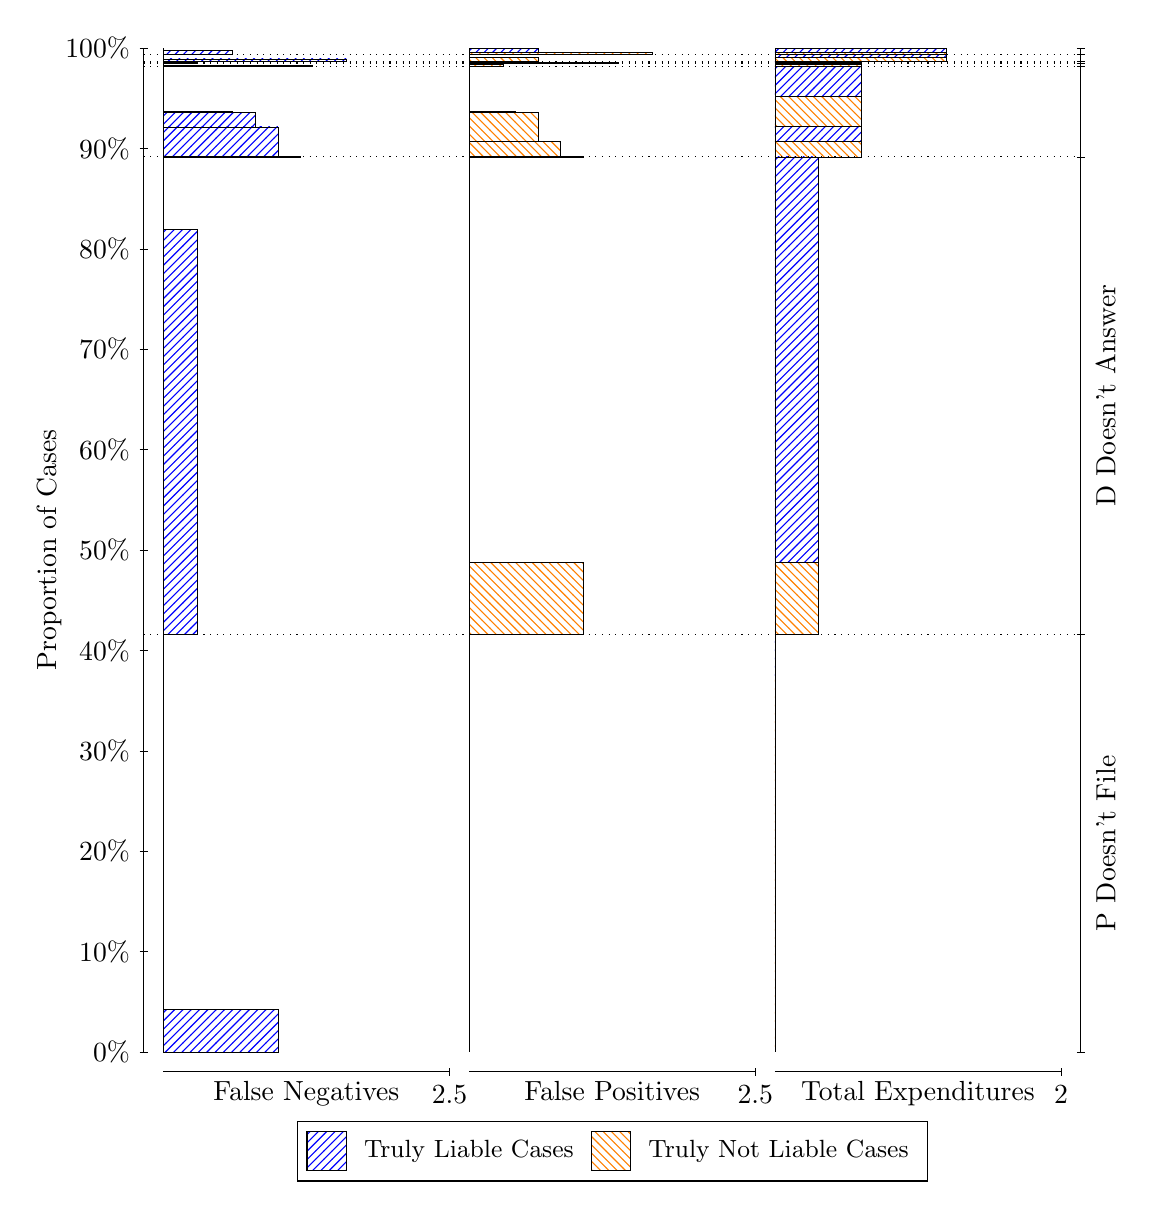
\begin{tikzpicture}
\draw[black, very thin] (1.5,1.75) -- (1.5,14.5);
\node[rotate=90, text=black, anchor=center] at (0.3, 8.125) {Proportion of Cases};
\draw[black, very thin] (1.45,1.75) -- (1.55,1.75);
\node[text=black, anchor=east] at (1.45, 1.75) {0\%};
\draw[black, very thin] (1.45,3.025) -- (1.55,3.025);
\node[text=black, anchor=east] at (1.45, 3.025) {10\%};
\draw[black, very thin] (1.45,4.3) -- (1.55,4.3);
\node[text=black, anchor=east] at (1.45, 4.3) {20\%};
\draw[black, very thin] (1.45,5.575) -- (1.55,5.575);
\node[text=black, anchor=east] at (1.45, 5.575) {30\%};
\draw[black, very thin] (1.45,6.85) -- (1.55,6.85);
\node[text=black, anchor=east] at (1.45, 6.85) {40\%};
\draw[black, very thin] (1.45,8.125) -- (1.55,8.125);
\node[text=black, anchor=east] at (1.45, 8.125) {50\%};
\draw[black, very thin] (1.45,9.4) -- (1.55,9.4);
\node[text=black, anchor=east] at (1.45, 9.4) {60\%};
\draw[black, very thin] (1.45,10.675) -- (1.55,10.675);
\node[text=black, anchor=east] at (1.45, 10.675) {70\%};
\draw[black, very thin] (1.45,11.95) -- (1.55,11.95);
\node[text=black, anchor=east] at (1.45, 11.95) {80\%};
\draw[black, very thin] (1.45,13.225) -- (1.55,13.225);
\node[text=black, anchor=east] at (1.45, 13.225) {90\%};
\draw[black, very thin] (1.45,14.5) -- (1.55,14.5);
\node[text=black, anchor=east] at (1.45, 14.5) {100\%};

\draw[black, very thin] (13.4,1.75) -- (13.4,14.5);
\draw[black, very thin] (13.35,1.75) -- (13.45,1.75);
\node[anchor=west] at (13.35, 1.75) {};
\draw[black, very thin] (13.35,7.0516) -- (13.45,7.0516);
\node[anchor=west] at (13.35, 7.0516) {};
\draw[black, very thin] (13.35,13.118) -- (13.45,13.118);
\node[anchor=west] at (13.35, 13.118) {};
\draw[black, very thin] (13.35,14.265) -- (13.45,14.265);
\node[anchor=west] at (13.35, 14.265) {};
\draw[black, very thin] (13.35,14.31) -- (13.45,14.31);
\node[anchor=west] at (13.35, 14.31) {};
\draw[black, very thin] (13.35,14.327) -- (13.45,14.327);
\node[anchor=west] at (13.35, 14.327) {};
\draw[black, very thin] (13.35,14.417) -- (13.45,14.417);
\node[anchor=west] at (13.35, 14.417) {};
\draw[black, very thin] (13.35,14.5) -- (13.45,14.5);
\node[anchor=west] at (13.35, 14.5) {};

\draw[black, very thin, pattern color=blue, pattern=north east lines] (1.75,1.75) rectangle (3.2033,2.2912);
\draw[black, very thin, pattern color=orange, pattern=north west lines] (1.75,2.2912) rectangle (1.75,7.0516);
\draw[black, very thin, pattern color=blue, pattern=north east lines] (1.75,7.0516) rectangle (2.186,12.201);
\draw[black, very thin, pattern color=orange, pattern=north west lines] (1.75,12.201) rectangle (1.75,13.118);
\draw[black, very thin, pattern color=blue, pattern=north east lines] (1.75,13.118) rectangle (3.494,13.123);
\draw[black, very thin, pattern color=blue, pattern=north east lines] (1.75,13.123) rectangle (3.2033,13.499);
\draw[black, very thin, pattern color=blue, pattern=north east lines] (1.75,13.499) rectangle (3.058,13.499);
\draw[black, very thin, pattern color=blue, pattern=north east lines] (1.75,13.499) rectangle (2.9127,13.687);
\draw[black, very thin, pattern color=blue, pattern=north east lines] (1.75,13.687) rectangle (2.622,13.691);
\draw[black, very thin, pattern color=orange, pattern=north west lines] (1.75,13.691) rectangle (1.75,14.265);
\draw[black, very thin, pattern color=blue, pattern=north east lines] (1.75,14.265) rectangle (3.6393,14.282);
\draw[black, very thin, pattern color=orange, pattern=north west lines] (1.75,14.282) rectangle (1.75,14.31);
\draw[black, very thin, pattern color=blue, pattern=north east lines] (1.75,14.31) rectangle (2.186,14.321);
\draw[black, very thin, pattern color=orange, pattern=north west lines] (1.75,14.321) rectangle (1.75,14.327);
\draw[black, very thin, pattern color=blue, pattern=north east lines] (1.75,14.327) rectangle (4.0753,14.361);
\draw[black, very thin, pattern color=orange, pattern=north west lines] (1.75,14.361) rectangle (1.75,14.417);
\draw[black, very thin, pattern color=blue, pattern=north east lines] (1.75,14.417) rectangle (2.622,14.467);
\draw[black, very thin, pattern color=orange, pattern=north west lines] (1.75,14.467) rectangle (1.75,14.5);
\draw[black, very thin, pattern color=orange, pattern=north west lines] (5.6333,1.75) rectangle (5.6333,6.5104);
\draw[black, very thin, pattern color=blue, pattern=north east lines] (5.6333,6.5104) rectangle (5.6333,7.0516);
\draw[black, very thin, pattern color=orange, pattern=north west lines] (5.6333,7.0516) rectangle (7.0867,7.9687);
\draw[black, very thin, pattern color=blue, pattern=north east lines] (5.6333,7.9687) rectangle (5.6333,13.118);
\draw[black, very thin, pattern color=orange, pattern=north west lines] (5.6333,13.118) rectangle (7.0867,13.122);
\draw[black, very thin, pattern color=orange, pattern=north west lines] (5.6333,13.122) rectangle (6.796,13.31);
\draw[black, very thin, pattern color=orange, pattern=north west lines] (5.6333,13.31) rectangle (6.6507,13.311);
\draw[black, very thin, pattern color=orange, pattern=north west lines] (5.6333,13.311) rectangle (6.5053,13.686);
\draw[black, very thin, pattern color=orange, pattern=north west lines] (5.6333,13.686) rectangle (6.2147,13.693);
\draw[black, very thin, pattern color=blue, pattern=north east lines] (5.6333,13.693) rectangle (5.6333,14.265);
\draw[black, very thin, pattern color=orange, pattern=north west lines] (5.6333,14.265) rectangle (6.0693,14.294);
\draw[black, very thin, pattern color=blue, pattern=north east lines] (5.6333,14.294) rectangle (5.6333,14.31);
\draw[black, very thin, pattern color=orange, pattern=north west lines] (5.6333,14.31) rectangle (7.5227,14.317);
\draw[black, very thin, pattern color=blue, pattern=north east lines] (5.6333,14.317) rectangle (6.0693,14.327);
\draw[black, very thin, pattern color=orange, pattern=north west lines] (5.6333,14.327) rectangle (6.5053,14.383);
\draw[black, very thin, pattern color=blue, pattern=north east lines] (5.6333,14.383) rectangle (5.6333,14.417);
\draw[black, very thin, pattern color=orange, pattern=north west lines] (5.6333,14.417) rectangle (7.9587,14.449);
\draw[black, very thin, pattern color=blue, pattern=north east lines] (5.6333,14.449) rectangle (6.5053,14.5);
\draw[black, very thin, pattern color=orange, pattern=north west lines] (9.5167,1.75) rectangle (9.5167,6.5104);
\draw[black, very thin, pattern color=blue, pattern=north east lines] (9.5167,6.5104) rectangle (9.5167,7.0516);
\draw[black, very thin, pattern color=orange, pattern=north west lines] (9.5167,7.0516) rectangle (10.062,7.9687);
\draw[black, very thin, pattern color=blue, pattern=north east lines] (9.5167,7.9687) rectangle (10.062,13.118);
\draw[black, very thin, pattern color=orange, pattern=north west lines] (9.5167,13.118) rectangle (10.607,13.31);
\draw[black, very thin, pattern color=blue, pattern=north east lines] (9.5167,13.31) rectangle (10.607,13.502);
\draw[black, very thin, pattern color=orange, pattern=north west lines] (9.5167,13.502) rectangle (10.607,13.884);
\draw[black, very thin, pattern color=blue, pattern=north east lines] (9.5167,13.884) rectangle (10.607,14.265);
\draw[black, very thin, pattern color=orange, pattern=north west lines] (9.5167,14.265) rectangle (10.607,14.294);
\draw[black, very thin, pattern color=blue, pattern=north east lines] (9.5167,14.294) rectangle (10.607,14.31);
\draw[black, very thin, pattern color=orange, pattern=north west lines] (9.5167,14.31) rectangle (10.607,14.317);
\draw[black, very thin, pattern color=blue, pattern=north east lines] (9.5167,14.317) rectangle (10.607,14.327);
\draw[black, very thin, pattern color=orange, pattern=north west lines] (9.5167,14.327) rectangle (11.697,14.383);
\draw[black, very thin, pattern color=blue, pattern=north east lines] (9.5167,14.383) rectangle (11.697,14.417);
\draw[black, very thin, pattern color=orange, pattern=north west lines] (9.5167,14.417) rectangle (11.697,14.449);
\draw[black, very thin, pattern color=blue, pattern=north east lines] (9.5167,14.449) rectangle (11.697,14.5);
\draw[black, dotted] (1.5,7.0516) -- (13.4,7.0516);
\draw[black, dotted] (1.5,13.118) -- (13.4,13.118);
\draw[black, dotted] (1.5,14.265) -- (13.4,14.265);
\draw[black, dotted] (1.5,14.31) -- (13.4,14.31);
\draw[black, dotted] (1.5,14.327) -- (13.4,14.327);
\draw[black, dotted] (1.5,14.417) -- (13.4,14.417);
\draw[black, very thin] (1.75,1.5) -- (5.3833,1.5);
\node[text=black, anchor=north] at (3.5667, 1.5) {False Negatives};
\draw[black, very thin] (5.3833,1.45) -- (5.3833,1.55);
\node[text=black, anchor=north] at (5.3833, 1.45) {2.5};

\draw[black, very thin] (5.6333,1.5) -- (9.2667,1.5);
\node[text=black, anchor=north] at (7.45, 1.5) {False Positives};
\draw[black, very thin] (9.2667,1.45) -- (9.2667,1.55);
\node[text=black, anchor=north] at (9.2667, 1.45) {2.5};

\draw[black, very thin] (9.5167,1.5) -- (13.15,1.5);
\node[text=black, anchor=north] at (11.333, 1.5) {Total Expenditures};
\draw[black, very thin] (13.15,1.45) -- (13.15,1.55);
\node[text=black, anchor=north] at (13.15, 1.45) {2};

\node[text=black, centered, rotate=90] at (13.72, 4.4008) {P Doesn't File};
\node[text=black, centered, rotate=90] at (13.72, 10.085) {D Doesn't Answer};






\draw (7.449999999999999,1.5) node[draw=none] (baseCoordinate) {};
\begin{scope}[align=center]
        \matrix[scale=0.5, draw=black, below=0.5cm of baseCoordinate, nodes={draw}, column sep=0.1cm]{
            \node[rectangle, draw, minimum width=0.5cm, minimum height=0.5cm, pattern color=blue, pattern=north east lines] {}; &
            \node[draw=none, font=\small, text=black] (B) {Truly Liable Cases}; &
            \node[rectangle, draw, minimum width=0.5cm, minimum height=0.5cm, pattern color=orange, pattern=north west lines] {}; &
            \node[draw=none, font=\small, text=black] (B) {Truly Not Liable Cases}; \\
            };
\end{scope}

\end{tikzpicture}
\end{document}